\section{Gesture Generation}
\label{sec:gesture_generation}
The generator module is the core component of our system. It synthesizes realistic gesture motions according to a sequence of gesture lexemes, the corresponding style codes, and the low-level features of the audio. In this section, we first introduce how we construct the gesture lexicon and then describe the design and training of the gesture generator.

\subsection{Construction of Gesture Lexicon}
\label{subsec:gesture_style_embedding}
As revealed in several pieces of literature in linguistics \cite{Neff2008Gesture,Kipp2004_Gesture,Webb1996_Linguistic}, only a limited number of lexemes are used in everyday conversation. We assume that each lexeme corresponds to a specific motion category. Our goal is then to extract those motion categories from a large gesture dataset. To achieve this goal, we employ the vector quantized variational autoencoder (VQ-VAE) model \cite{oord2017neural} to learn a categorical representation of the motion and construct the gesture lexicon.

VQ-VAE has been widely used to learn categorical spaces in many successful temporal models \cite{prafulla2020jukebox, baevski2020vq-wav2vec, yan2021videogpt,ramesh2021DALLE}. Similar to a regular autoencoder, a VQ-VAE also has an encoder-decoder structure but quantizes the latent space using a discrete codebook. The codebook consists of a list of vectors and their associated indices. The output of the encoder network is compared to every vector in the codebook, where the vector that is the closest in Euclidean distance is considered to be the latent representation of the input and will be fed to the decoder. The training of a VQ-VAE is achieved by pulling together the latent code of input and its corresponding codebook vector.

As illustrated in \fig\ref{fig:system_overview}, we construct the gesture lexicon by learning the categorical representations of the normalized motion blocks using VQ-VAE. Following \cite{oord2017neural}, the loss function is defined as
\begin{align}
    \mathcal{L}_{\eqword{lexicon}} &= \lVert \vect{M}-\mathcal{D}({\vect{s}}) \rVert_2^2 \nonumber\\
    &+  w_{\alpha}\lVert \mathcal{E}(\vect{M}) -\stopgrad({\vect{s}}) \rVert_2^2 
    +  w_{\beta}\lVert \stopgrad(\mathcal{E}(\vect{M})) - {\vect{s}} \rVert_2^2,
    \label{eqn:vq_vae_loss}
\end{align}
where
\begin{equation}
    {\vect{s}} = \argmin_{\vect{s}'\in \mathcal{S}} \lVert \vect{s}' - \mathcal{E}(\vect{M}) \rVert_2, \label{eqn:codebook_lookup}
\end{equation}
$\vect{M}$ is a normalized motion block, $\mathcal{E}$ and $\mathcal{D}$ represent the encoder and decoder, respectively, $\stopgrad$ stands for the \emph{stop gradient} operator that prevents the gradient from backpropagating through it, $\mathcal{S}$ represents the codebook, or the lexicon, and $\vect{s}$ is a codebook vector, or a lexeme. The first term of \eqn\eqref{eqn:vq_vae_loss} penalizes the reconstruction error, while the other two terms pull together the latent representation of motion $\vect{M}$ and its corresponding lexeme. Notably, since $\mathcal{S}$ is discrete, the $\argmin$ operator in \eqn\eqref{eqn:codebook_lookup} does not generate a gradient. The gradient of the reconstruction error with respect to the latent code is passed unaltered to the encoder during the backward pass as suggested in~\cite{oord2017neural}.
%
\begin{figure}[t]
    \centering
    \begin{subfigure}[t]{0.47\linewidth}
        \centering
        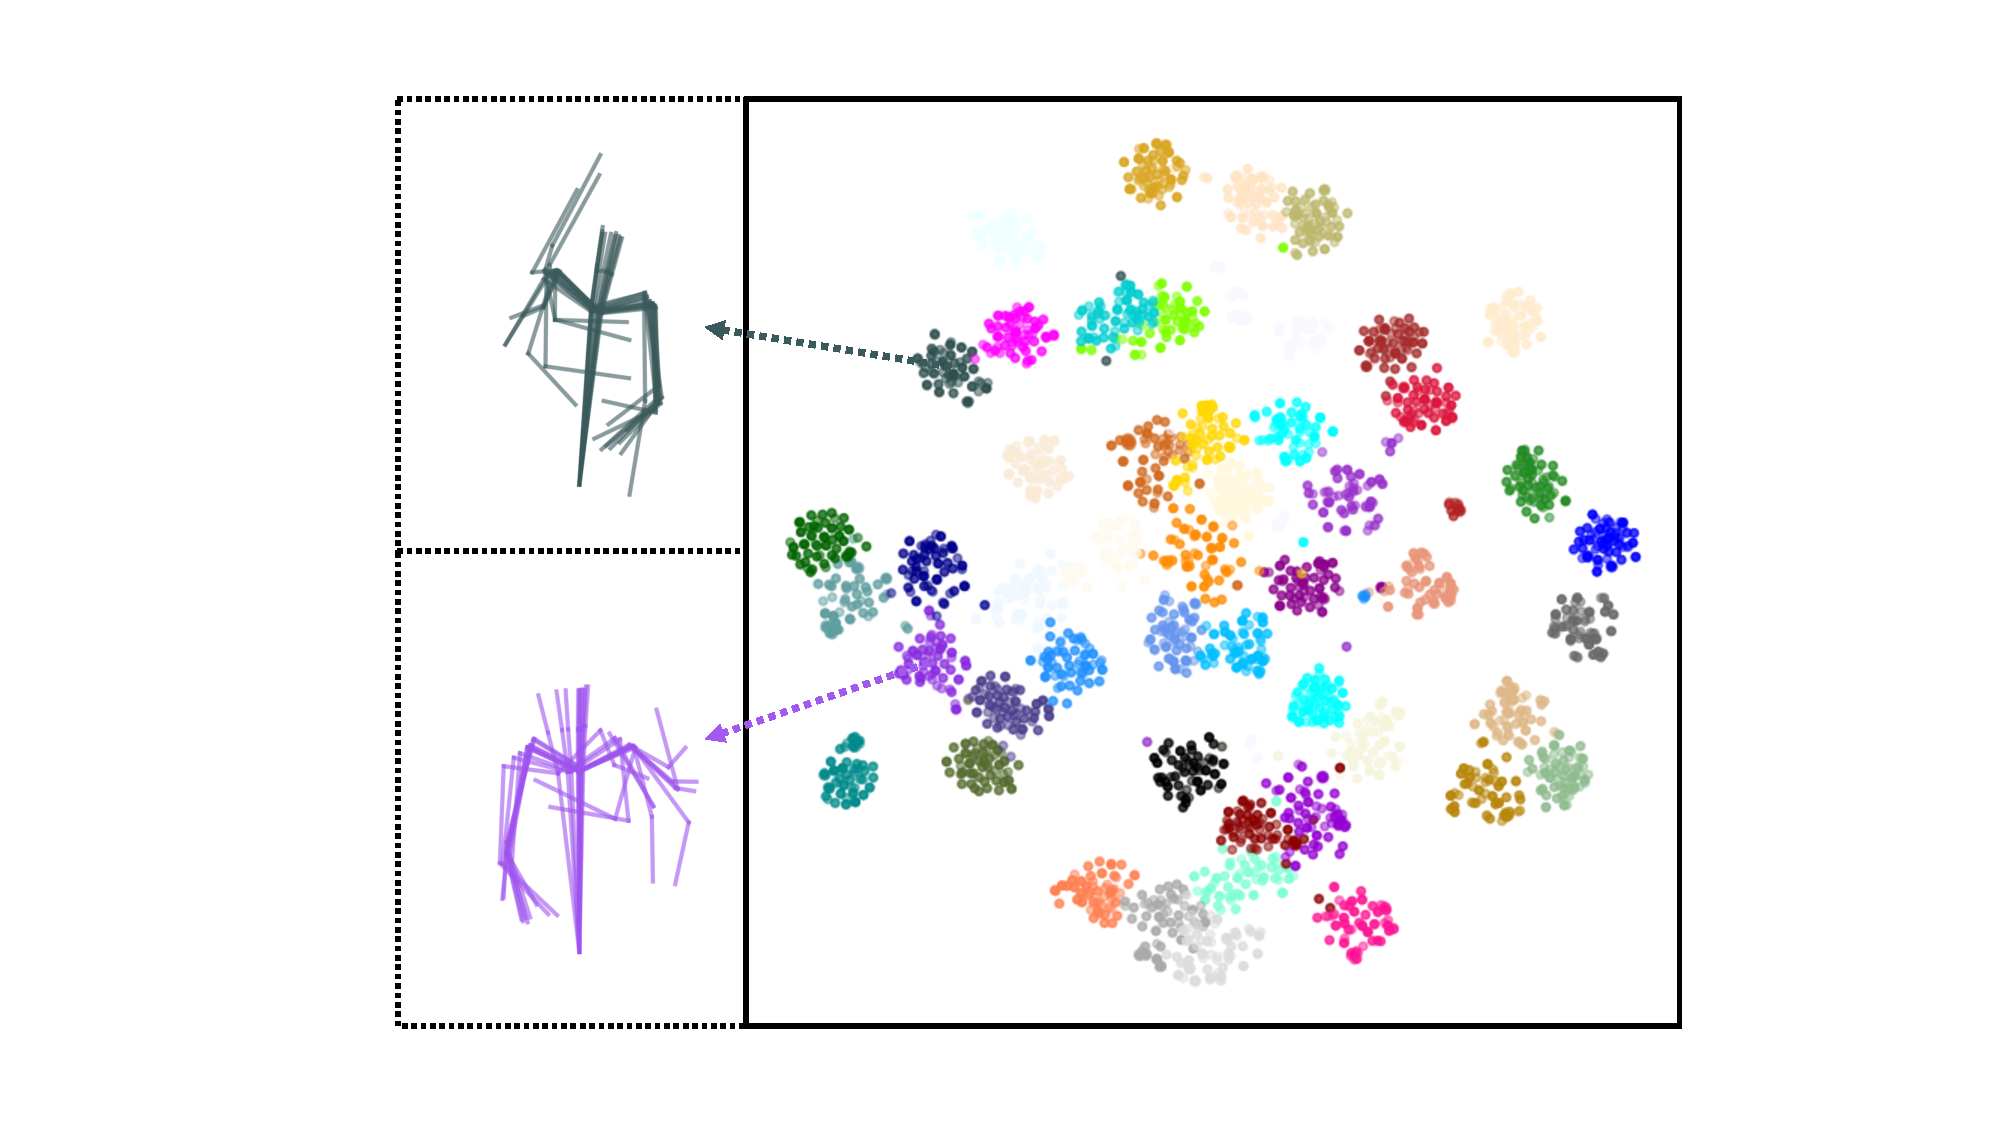
\includegraphics[width=\linewidth]{figures/fig3a.pdf}
        \caption{Trinity Gesture dataset.}
        % \label{fig:fig3a}
    \end{subfigure}
    \hspace{\fill}
    \begin{subfigure}[t]{0.47\linewidth}
        \centering
        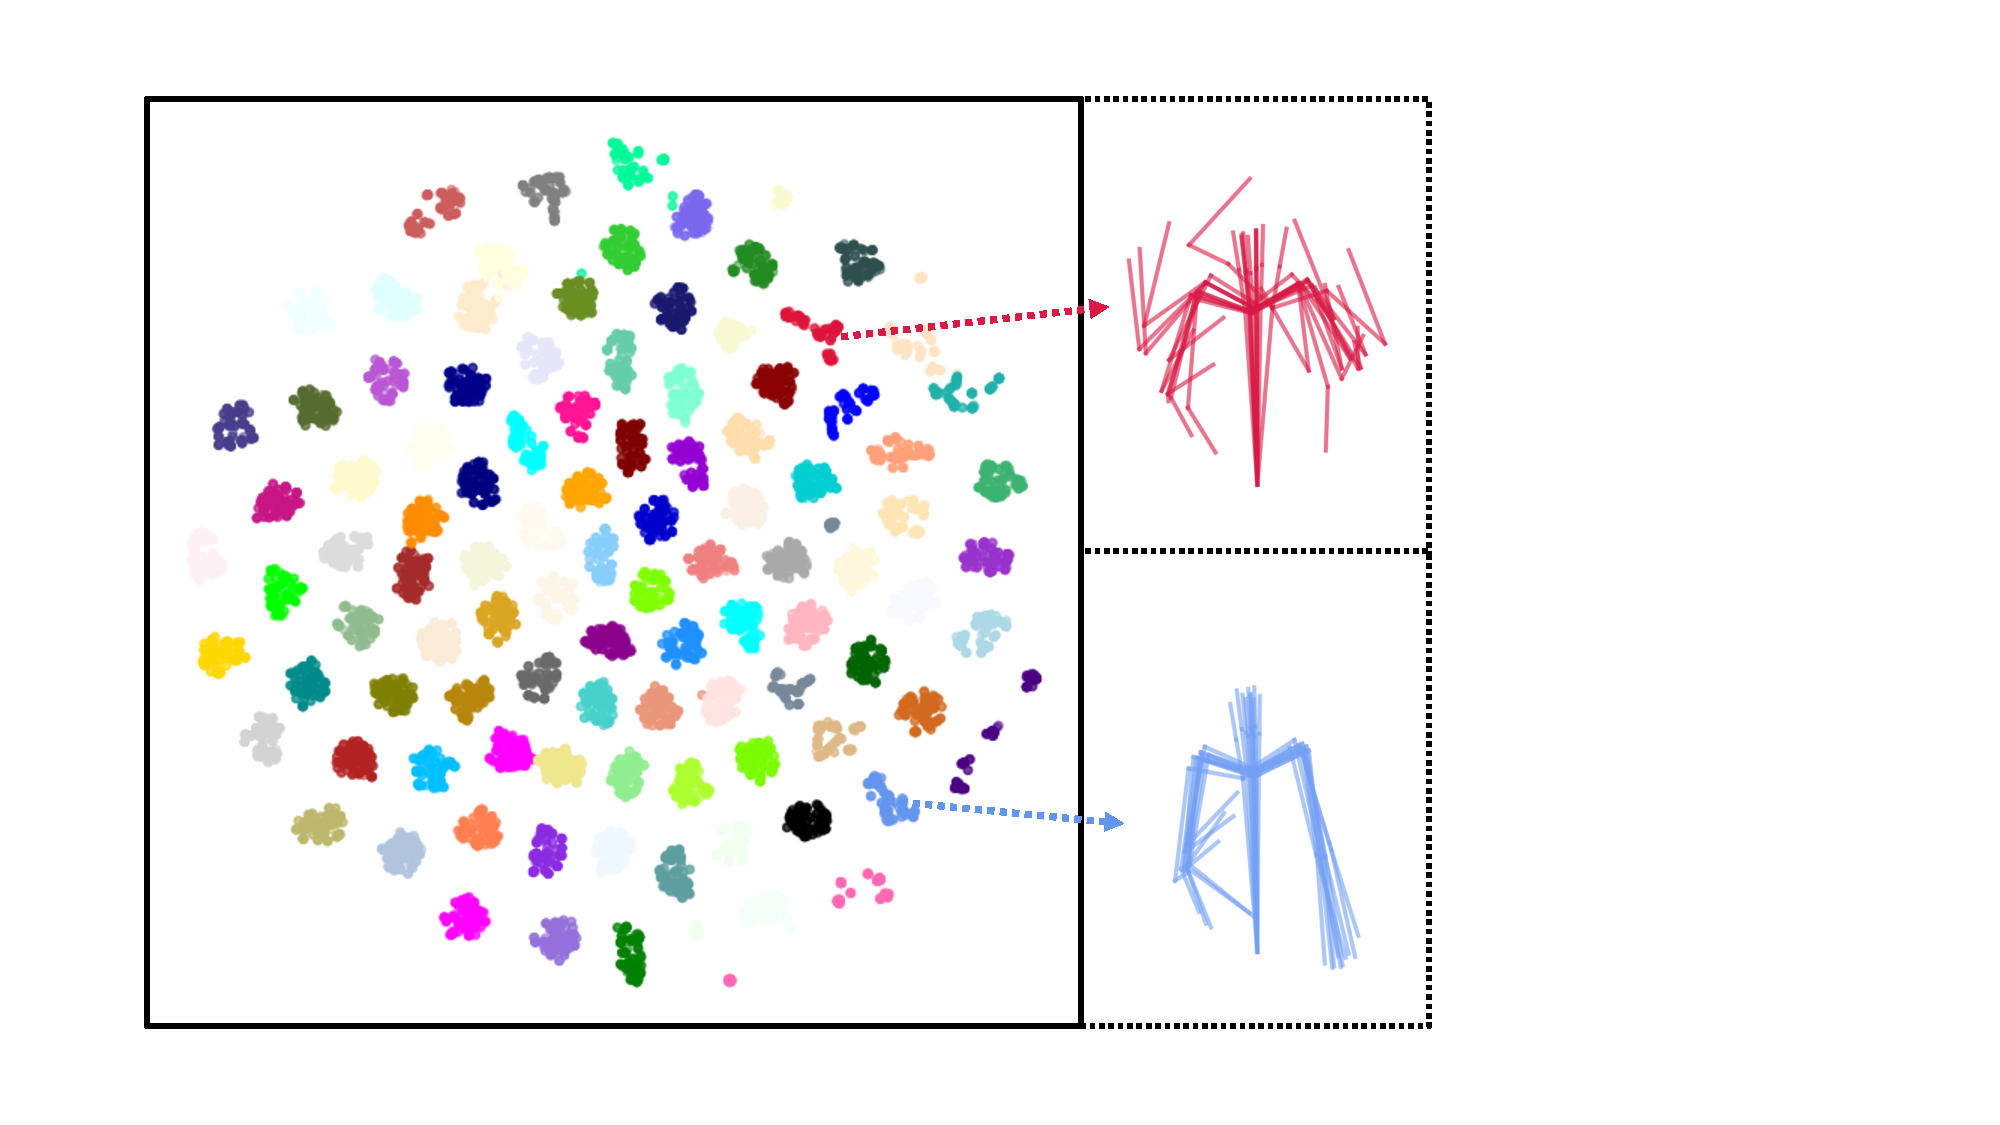
\includegraphics[width=\linewidth]{figures/fig3b.pdf}
        \caption{TED Gesture dataset.}
        % \label{fig:fig3b}
    \end{subfigure}
    \caption{t-SNE visualization of gesture lexicons. Each color stands for a gesture lexeme. (a) lexicon learned on the Trinity Gesture dataset with 50 lexemes. (b) lexicon learned on the TED Gesture dataset with 100 lexemes.}
    \Description{}
    \label{fig:gesture_lexicon}
\end{figure}

We train the VQ-VAE on each dataset in a separate pre-training stage. The encoder is a multi-layer network consisting of four 1-D convolutional layers followed by a fully connected layer, which encodes a motion block into a vector $\vect{s}\in\mathbb{R}^{d_s}$. The decoder is a mirror of the encoder structurally. The size of the lexicon is a hyperparameter, which is chosen empirically based on the size and complexity of the dataset. \fig\ref{fig:gesture_lexicon} shows the t-SNE visualization of the training results on two speech-gesture datasets, along with sample gestures of several lexemes. Once learned, the gesture lexicon and the gesture lexeme of every motion block are fixed and used by the generator and interpreters in both the training and inference stages.

\subsection{Architecture of Generator}
As illustrated in \fig\ref{fig:system_overview}, the generator module of our system is an autoregressive encoder-decoder network, where a new motion block is conditioned on not only the input speech but also the preceding block, the gesture lexeme, and the style code. More specifically, the generation of a motion block $\vect{M}_{i}$ can be formulated as
\begin{equation}
    \vect{M}_{i}^*=\mathcal{G}(\tildevect{M}_{i-1},\tildevect{A}_{i},\vect{s}_i,\vect{z}_i,\vect{P}) \label{eqn:generator_block},
\end{equation}
where $\tildevect{M}_{i-1}$ represents the features extracted from the preceding motion block, $\tildevect{A}_{i}$ stands for the representation of the input audio, $\vect{s}_i$ and $\vect{z}_i$ are the gesture lexeme and style code of the new block, respectively. Note that we use an asterisk~($*$) to indicate a generated quantity. All these motion and feature blocks have the same length of $K$ frames, where $\vect{s}_i$ and $\vect{z}_i$ are repeated and stacked into the corresponding blocks, represented as $\vect{S}_i$ and $\vect{Z}_i$, respectively.

We extract the motion feature $\tildevect{M}_{i-1}\in\mathbb{R}^{K\times{}d_{\tilde{m}}}$ as 
\begin{equation}
    \tildevect{M}_{i-1} = \mathcal{E}_M(\vect{M}_{i-1}),
\end{equation}
where the encoder $\mathcal{E}_M$ is a 1-D convolutional network with three layers.
%
The audio feature $\tildevect{A}_{i}\in\mathbb{R}^{K\times{}d_{\tilde{a}}}$ is computed using three consecutive audio blocks
\begin{equation}
    \tildevect{A}_{i} = \mathcal{E}_A(\vect{A}^{\eqword{low}}_{i-1},\vect{A}^{\eqword{low}}_{i},\vect{A}^{\eqword{low}}_{i+1})
\end{equation}
to allow the generator to prepare for the future gestures. 
Notably, the original duration of an audio block is characterized by the onset interval $[D_m, D_M]$, which is typically $[0.2s, 0.5s]$ in our experiments. Thus the temporal window of this encoder is roughly $[0.6s, 1.5s]$.
Each $\vect{A}^{\eqword{low}}$ is the low-level feature pre-computed from the raw speech audio. We assume that $\vect{A}^{\eqword{low}}$ already captures necessary information and use a simple network consisting of one fully connected layer as the encoder $\mathcal{E}_A$.

In the training stage, the gesture lexeme $\vect{s}_i$ of each motion block is determined during the construction of the gesture lexicon, while the style code $\vect{z}_i$ is a learnable variable that will be trained along with the generator. In the inference stage, both $\vect{s}_i$ and $\vect{z}_i$ are provided by the interpreters, as will be discussed below.

In addition to these features, we include a positional encoding block, $\vect{P}\in\mathbb{R}^{K\times{}d_{P}}$, to let the generator know the progress of the generation in a motion block, which is a standard component of transformers~\cite{Vaswani2017_Attentiona} and many sequence generation tasks~\cite{Harvey2020_motionInBetween}. For our normalized blocks with $K$ frames, we compute $\vect{P}=\{\vect{p}_1,\dots,\vect{p}_K\}$ as
\begin{align}
    \vect{p}_{2k} = \sin\left(\frac{K}{\beta^{2k/d_{P}}}\right) \quad
    \vect{p}_{2k+1} = \cos\left(\frac{K}{\beta^{2k/d_{P}}}\right),
    \label{eqn:pos_enc}
\end{align}
where $d_{P}$ is the dimension of the encoding and $\beta=10,000$ is a constant controlling the rate of change in frequencies along the embedding dimensions.

The generator $\mathcal{G}$ consists of an MLP-based encoder followed by an LSTM-based decoding network. Inspired by the successful systems in generating sequential output \cite{richard2021meshtalk,oord2017neural}, we quantized the latent space of the encoder into $H$ groups of $C$-way categories, which provides $C^H$ different configurations. We use $H=64$ and $C=128$ to ensure a large enough categorical space. In addition, we leverage Gumbel-softmax~\cite{jang2017categorical} to convert a latent code into a codebook vector, which can be viewed as a differentiable sampling operator for the discrete codebook search.

\subsection{Training}
We train the generator $\mathcal{G}$, the encoders $\mathcal{E}_M$ and $\mathcal{E}_A$, and the learnable style codes $\{\vect{z}_i\}$ by minimizing a combination of loss terms:
\begin{equation}
    \mathcal{L}_{\eqword{gen}} 
    = w_{\eqword{rec}}\mathcal{L}_{\eqword{rec}}
    + w_{\eqword{perc}}\mathcal{L}_{\eqword{perc}}
    + w_{\eqword{lexeme}}\mathcal{L}_{\eqword{lexeme}}
    + w_{{z}}\mathcal{L}_{{z}}.\label{eqn:generator_loss}
\end{equation}
The reconstruction loss 
\begin{equation}
    \mathcal{L}_{\eqword{rec}}=\lVert \vect{M}_i - \vect{M}_i^* \rVert_2^2   
\end{equation}
is simply the MSE loss between the generated motion block and the ground truth. We additionally include a perceptual loss to ensure the similarity between the generated motion and the ground truth in the feature level as well, which is defined as
\begin{equation}
    \mathcal{L}_{\eqword{perc}} = \lVert \mathcal{E}(\vect{M}_i) - \mathcal{E}(\vect{M}_i^*) \rVert_2^2 ,
\end{equation}
where $\mathcal{E}$ is the motion encoder pre-trained in Section~\ref{subsec:gesture_style_embedding}.

We assume that the gesture lexeme determines the type of gesture motion, and the other speech modalities only affect the motion variations. To enforce this assumption, we develop a new perceptual loss, namely the lexeme loss. We first generate a number of new motion blocks using the current gesture lexeme but random sets of other features, 
\begin{equation}
    \vect{M}^{*}_j = \mathcal{G}(\tildevect{M}_{j-1}, \tildevect{A}_{j}, \vect{s}_i, \vect{z}_j, \vect{P}) ,
\end{equation}
where $\tildevect{M}_{j-1}$, $\tildevect{A}_{j}$, and $\vect{z}_j$ correspond to a random speech block $j$. Then the lexeme loss is defined as 
\begin{equation}
    \mathcal{L}_{\eqword{lexeme}}=\frac{1}{N_J}\sum_{j\in{}J}\lVert \vect{s}_i - \mathcal{E}(\vect{M}_j^*) \rVert_2^2 ,
\end{equation}
where $J$ is a random subset of all the motion blocks in the training dataset. The size of $J$, $N_J$, is chosen based on the size of the dataset.

Lastly, we regularize the learning of the style code by applying a KL-divergence loss
\begin{equation}
    \mathcal{L}_{z} = D_{KL}(\mathcal{N}(\mu_z, \sigma^2_z) \Vert \mathcal{N}(0, 1)),
\end{equation}
where $\mu_z$ and $\sigma^2_z$ are the mean and variance vectors of the style codes in a mini-batch, respectively.